\chapter{WG model Utilized in RSCAD and PowerFactory}\label{Appendix_A}

\section{RSCAD model}

The Type-4 \gls{WG} model is utilized for this thesis work, and the complete implementation of the model is described in this section. 

The \gls{PMSG} modelled in the small time step block, consists of the parameters shown in Figure \ref{fig:PMSG_block_para}. The \gls{PMSG} component majorly operates in two modes: Speed or Lock mode (LCKFR = 0) ; Torque or Free mode (LCKFR = 1).
As the name suggests, a control signal directly controls the speed of the machine in speed mode, and a control signal directly controls the torque of the machine in torque mode.  

\begin{figure}[H]
\centering
%\hspace*{-1.2cm}
    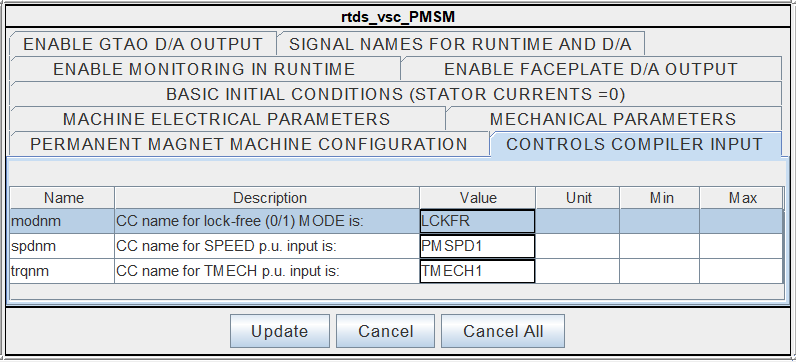
\includegraphics[height = 5cm,width = 11.5cm]{Diagrams/Appendix_A/PMSG_block_para.PNG}
    \caption{PMSG data}
    \label{fig:PMSG_block_para}
\end{figure}

The major three blocks that represent the control system of Type-4 \gls{WG} are:
\begin{itemize}
    \item Aerodynamic model
    \item Machine Side Converter model
    \item Grid Side Converter model
\end{itemize}

\section{Aerodynamic model}

\begin{figure}[]
\centering
%\hspace*{-1.2cm}
    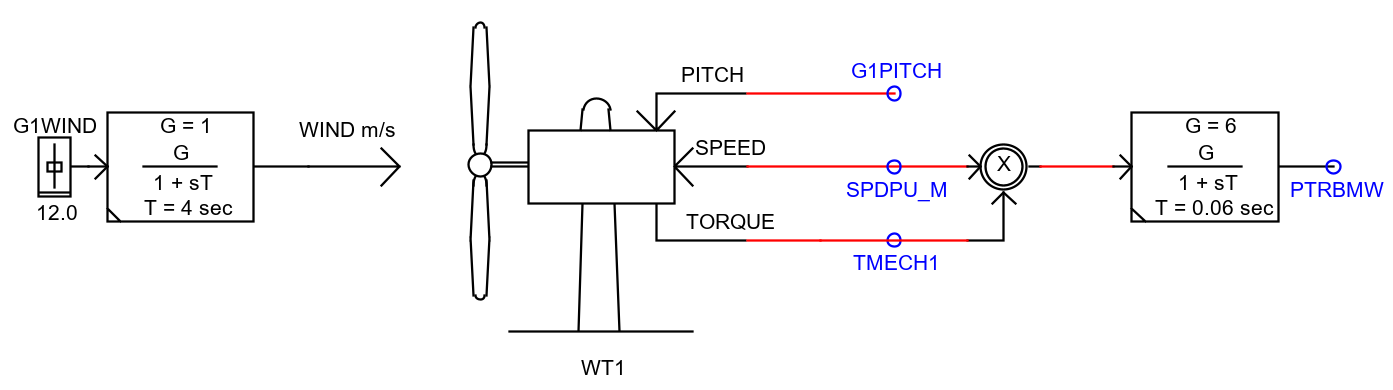
\includegraphics[height = 4.5cm,width = 15.5cm]{Diagrams/Appendix_A/Aerodynamic_model.PNG}
    \caption{Aerodynamic model}
    \label{fig:Aerodynamic_model}
\end{figure}

The aerodynamic block consists mainly of the wind turbine data and the coefficient data i.e. is the $C_p(\lambda,\beta)$ parameters, as shown in Figures \ref{fig:Turbine_data} and \ref{fig:Coeff_type}. The parameters used are for a 6 MVA rated \gls{WG} model. The detailed configuration of the aforementioned parameters is described in "WTG50R3.pdf" in the Samples folder in RSCAD. The aerodynamic model consists of the two mass representation model of \gls{WG} shown in Figure \ref{fig:Two-mass model}, and the pitch angle control is shown in Figure \ref{fig:Pitch_controller}. 

\begin{figure}[H]
\centering
%\hspace*{-1.2cm}
\begin{subfigure}{.55\textwidth}
  \centering
  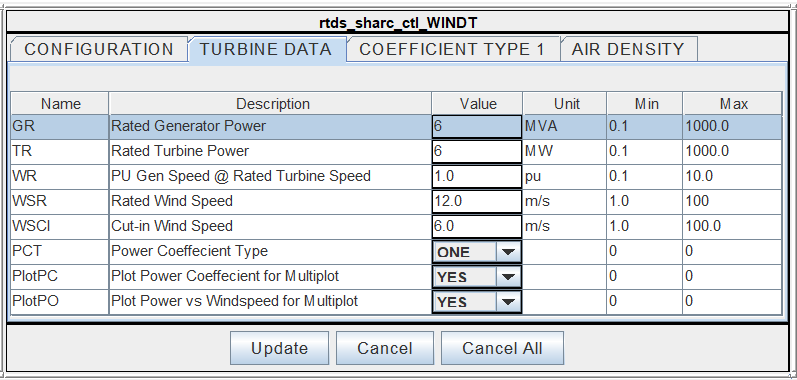
\includegraphics[height=4.5cm,width=8.5cm]{Diagrams/Appendix_A/Turbine_data.PNG}
  \caption{Turbine data}
  \label{fig:Turbine_data}
\end{subfigure}%
\begin{subfigure}{.45\textwidth}
  \centering
  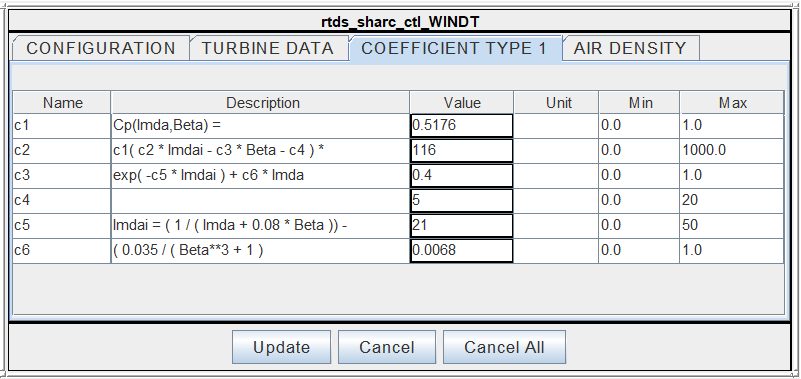
\includegraphics[height=4.5cm,width=8.5cm]{Diagrams/Appendix_A/Coeff_type.PNG}
  \caption{Coefficient data}
  \label{fig:Coeff_type}
\end{subfigure}
\caption{Aerodynamic model data}
\label{fig:aerodynamic_model_data}
\end{figure}

The inputs for the two-mass model are the mechanical torque from the aerodynamic model and the electrical torque from \gls{PMSG}. The output is the change in rotor speed ($SPDPU\_M$) and the generator speed ($SPDPU$). The two-mass model represents the non-linear nature of the wind turbine aerodynamics. To protect the turbines from damage due to high wind speeds, the pitch control mechanism is adapted. The maximum speed is controlled through the limits of the $G1MXPSD$ parameter. When the speed goes beyond the limit, a pitch angle ($G1PITCH$) is calculated, and this is provided as input to the aerodynamic model to compute a new speed.  

\begin{figure}[H]
\centering
%\hspace*{-1.2cm}
    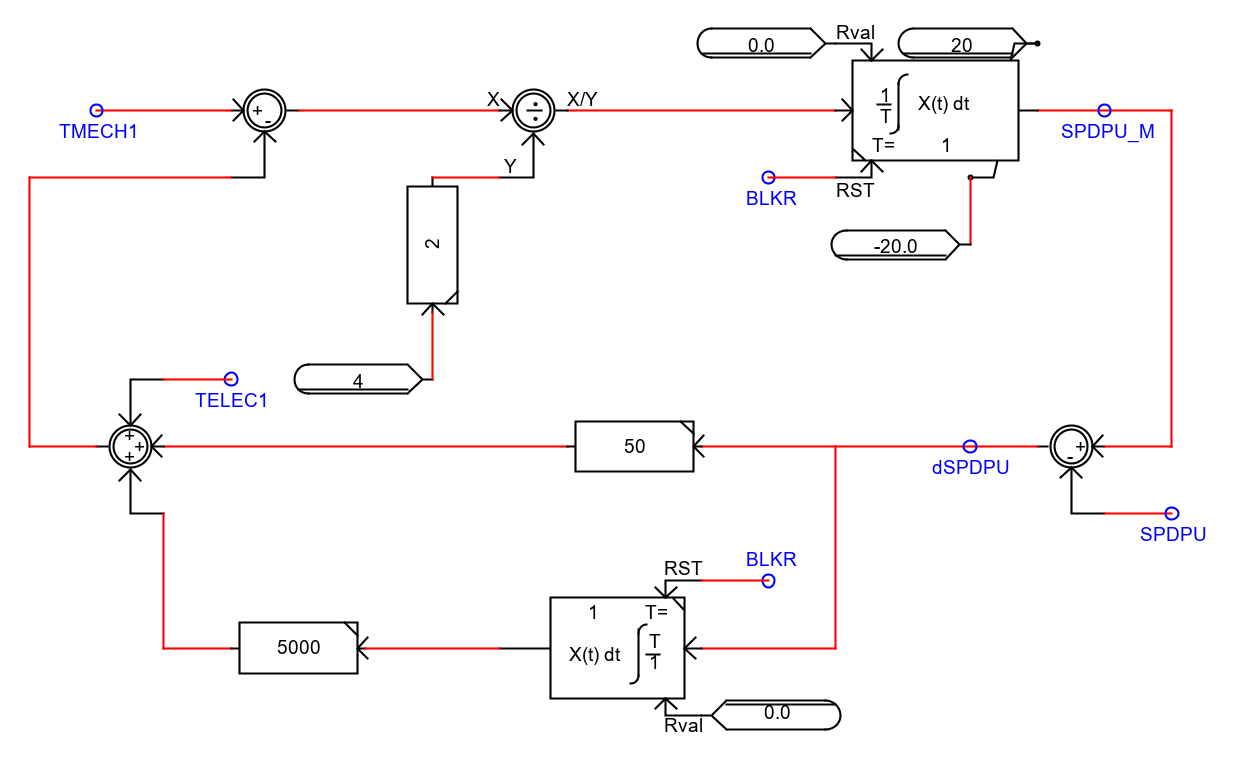
\includegraphics[height = 8.5cm,width = 12.5cm]{Diagrams/Appendix_A/Two_mass_model.PNG}
    \caption{Two-mass model}
    \label{fig:Two-mass model}
\end{figure}

\begin{figure}[H]
\centering
%\hspace*{-1.2cm}
    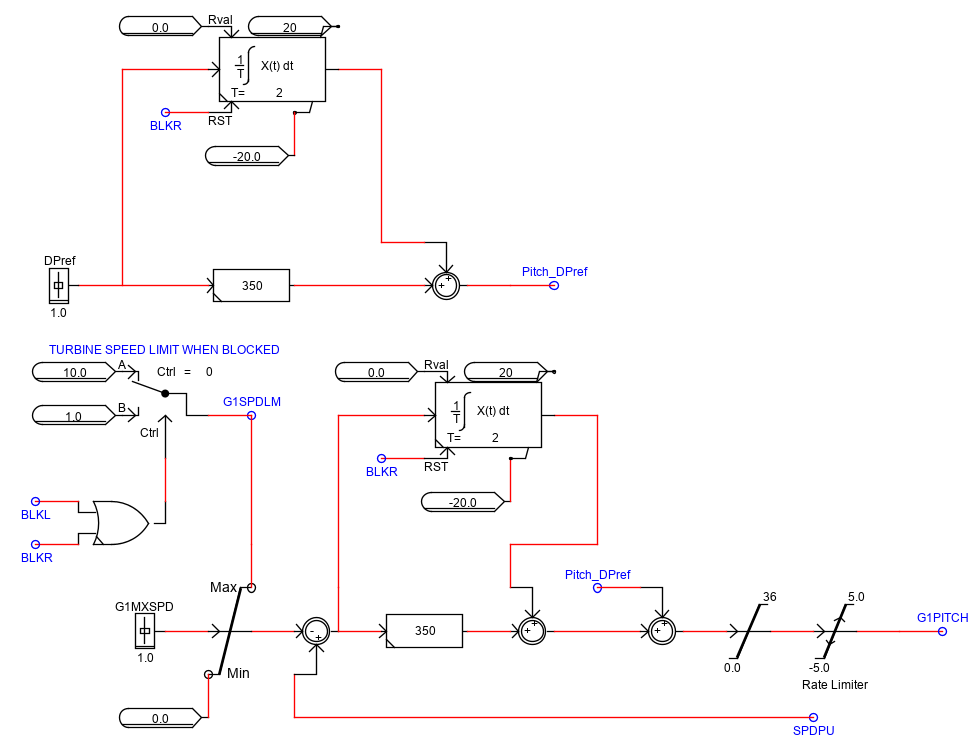
\includegraphics[height = 11.5cm,width = 14.5cm]{Diagrams/Appendix_A/Pitch_controller.PNG}
    \caption{Pitch angle control}
    \label{fig:Pitch_controller}
\end{figure}

\section{Machine Side Converter model}\label{MSC_Control}

The overall \gls{MSC} control is depicted, as shown in Figure \ref{fig:MSC_Control}. A three-level \gls{VSC} is used for operation as \gls{MSC} in this model. The conventional vector current control utilized in the \gls{MSC} control. As required for \gls{PI} control operation, the abc signals are transformed to the \gls{dq} frame using the rotor angle measurement for alignment and synchronizing with the \gls{dq} reference frame. The \gls{MSC} control consists of two inner fast control loops using \gls{PI} controllers that regulate the converter currents during all conditions, i.e. steady-state and dynamic scenarios. The reference values for the inner control loop is provided by the outer control loop. By measurement of active power of the \gls{WG}, a \gls{MPPT} control is used to output an optimum speed reference ($WMOPTPU$) as shown in Figure \ref{fig:MPPT_control}. The error difference from the optimum speed reference and the rotor speed is regulated through an outer \gls{PI} control loop. The modulation index for the \gls{MSC} control is same as \gls{GSC} control and is given by Equation \ref{MI_eq}.

\begin{figure}[H]
\centering
%\hspace*{-1.2cm}
    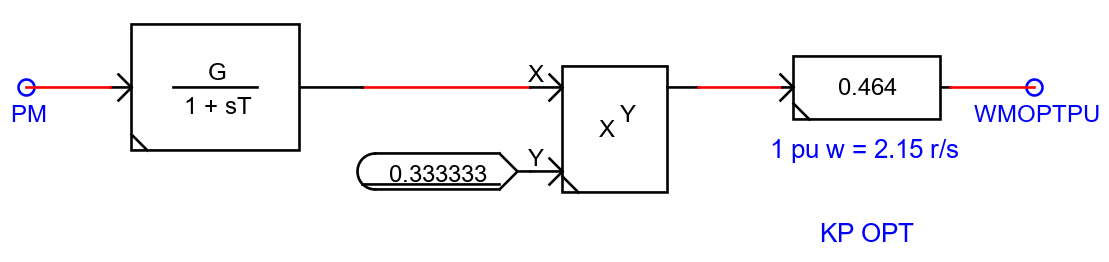
\includegraphics[height = 2.5cm,width = 9.5cm]{Diagrams/Appendix_A/MPPT_control.PNG}
    \caption{MPPT controller}
    \label{fig:MPPT_control}
\end{figure}

The gating for the \gls{MSC} control utilizes \gls{PWM} and the inputs for the triangular wave repeater in terms of point and slope, in the small time step environment are defined as shown in Figure \ref{fig:Triangular_wave_input}. However, the rated frequency of the \gls{PMSG} is chosen to be 3.77 Hz, and the frequency of the carrier wave is 31 times this frequency. Hence the slope of the triangular signal is double the carrier frequency which is then sent to the small time step block.  

\begin{figure}[H]
\text{\rotatebox{90}{\hspace{5mm}
\noindent
{\color{green} \rule{10mm}{1mm} } Outer control loop
\hspace{25mm}
\noindent
{\color{yellow} \rule{10mm}{1mm} } Inner control loop
\hspace{15mm}
\noindent
{\color{blue} \rule{10mm}{1mm} } Modulation limitation
\hspace{15mm}
\noindent
{\color{orange} \rule{10mm}{1mm} } Modulation index
}
\hspace{10mm}}
\centering
%\hspace*{-1.2cm}
    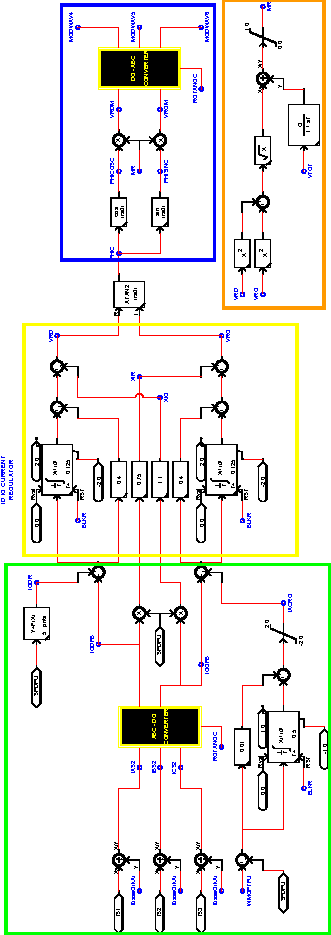
\includegraphics[height = 22cm,width = 7.5cm]{Diagrams/Appendix_A/MSC_control.pdf}
    \caption{MSC control}
    \label{fig:MSC_Control}
\end{figure}

\begin{figure}[H]
\centering
%\hspace*{-1.2cm}
    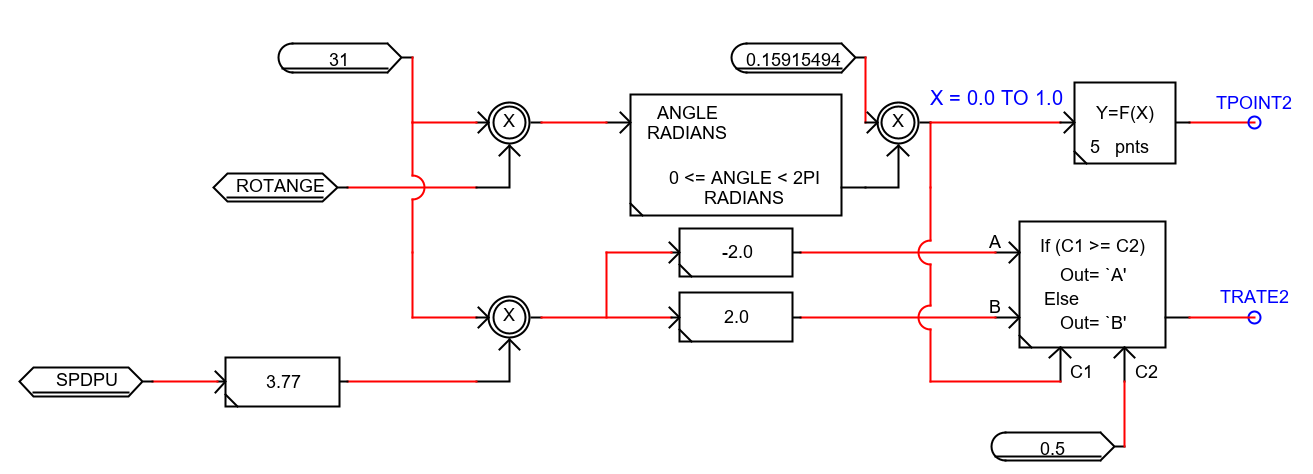
\includegraphics[height = 4.5cm,width = 12.5cm]{Diagrams/Appendix_A/Triangular_wave_input.PNG}
    \caption{Triangular wave inputs}
    \label{fig:Triangular_wave_input}
\end{figure}

The triangular wave repeater and the firing pulse generator blocks are placed in the small time step environment, as shown in Figure \ref{fig:Firing_blocks_MSC}. As the name suggests, the triangular wave repeater creates the triangular-carrier wave taking the points and slope as input and provides the carrier wave to the firing pulse generator. Each \gls{VSC} have dedicated firing pulse generator which takes the carrier wave input from the triangular wave repeater (e.g. TWAVE6) and the modulation signal from the large-time step block controls (e.g. MODWAV6). Depending on the comparison of these signals, the switching of the valves takes place. The firing signal to be sent to the \gls{VSC} leg are named for example FPOUT6. The number denomination for the three-phases of \gls{MSC} are 4,5 and 6 respectively in this model.  

\begin{figure}[H]
\centering
%\hspace*{-1.2cm}
    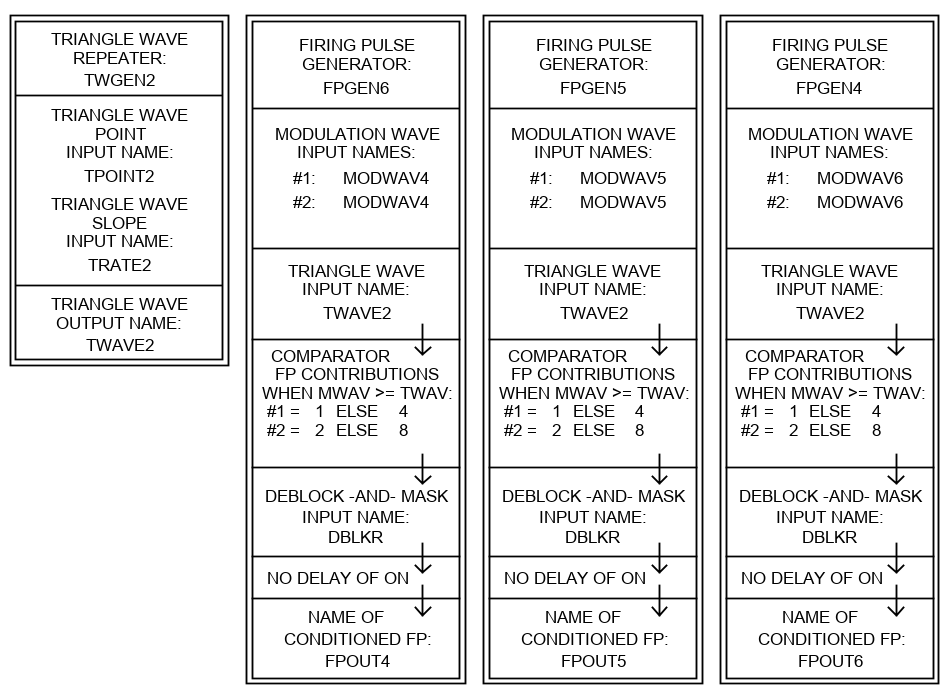
\includegraphics[height = 7.5cm,width = 9.5cm]{Diagrams/Appendix_A/Firing_blocks_MSC.PNG}
    \caption{Triangular wave repeater and Firing pulse generator for MSC}
    \label{fig:Firing_blocks_MSC}
\end{figure}

There exists a \gls{DC} link in between the \gls{MSC} and the \gls{GSC} consisting of capacitor banks on either end and a chopper circuit in between. The voltage in the upper and lower capacitive branches in the \gls{MSC} side is depicted as $V3$ and $V4$. Voltages in the branch at the \gls{GSC} side are $V1$ and $V2$. The voltages $V1$ and $V2$ sum up to $V_{DC\_ref}$ in the outer control loop for the \gls{GSC} as explained in Section \ref{Active_power_DVC_theory}. Hence, the control of d-axis voltage is associated with the control of active power, and this task is accomplished by regulating the \gls{DC} voltage. The voltage across the \gls{DC} link is maintained constant during steady state conditions. During the time of disturbance in the network, the chopper circuit gets activated and holds the \gls{DC} voltage within the limit. The chopper gets activated when the \gls{DC} voltage ($V1 + V2$) goes above 1.05 p.u. as shown in Figure \ref{fig:Chopper_circuit_signals}. The chopper also utilizes \gls{PWM} for gating and the signals involved are a 50 Hz carrier signal and, the difference between the maximum voltage limit (1.05 p.u. in this case) and the measured \gls{DC} voltage as the modulating signal. The triangular wave repeater block and the firing pulse generator block for the chopper is also placed in the small time step block and is shown in Figure \ref{fig:Chopper_circuit_firing}. The firing pulse output is provided to the circuit valve shown in Figure \ref{fig:Chopper_circuit}.

\begin{figure}[H]
\centering
%\hspace*{-1.2cm}
    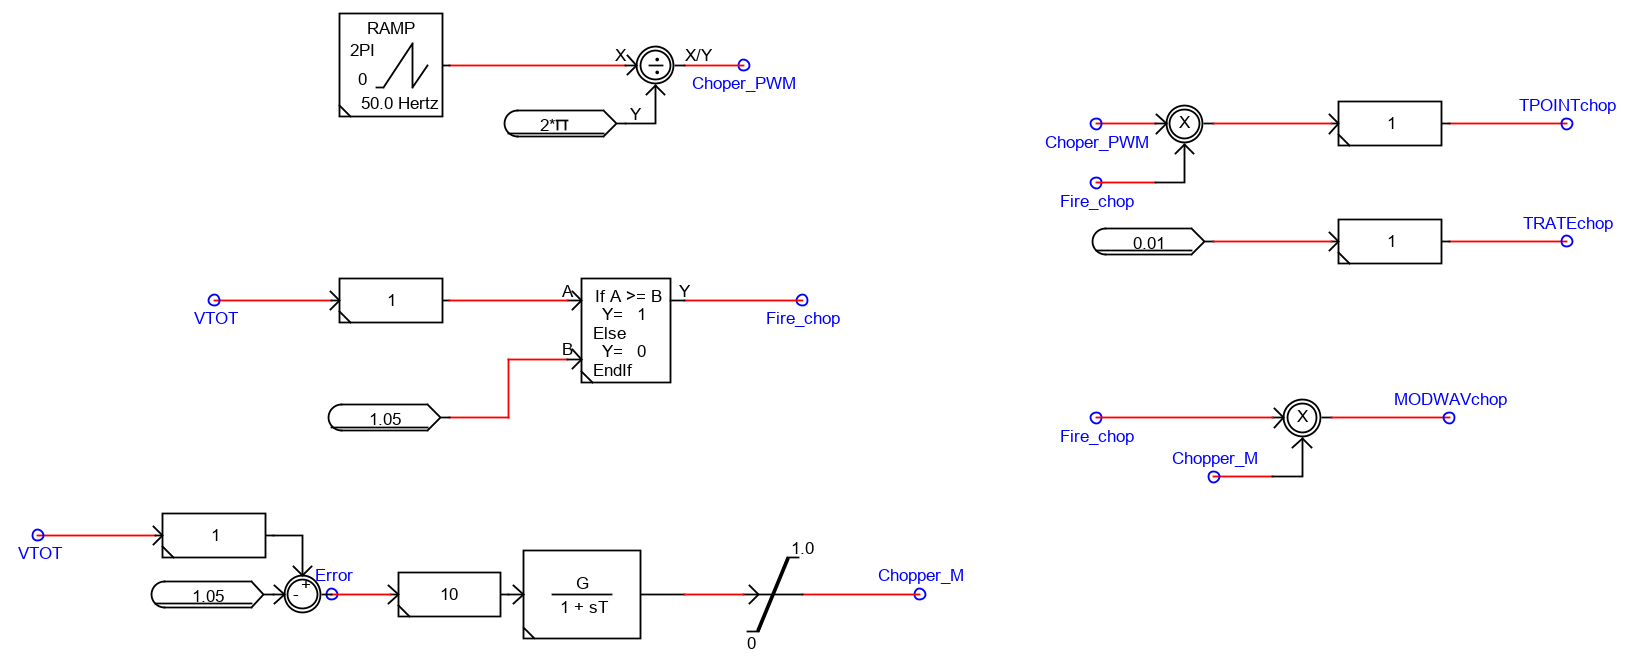
\includegraphics[height = 6.5cm,width = 16.5cm]{Diagrams/Appendix_A/Chopper_circuit_signals.PNG}
    \caption{Chopper activation control}
    \label{fig:Chopper_circuit_signals}
\end{figure}


\begin{figure}[H]
\centering
%\hspace*{-1.2cm}
\begin{subfigure}{.3\textwidth}
  \centering
  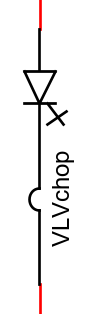
\includegraphics[height=4.5cm,width=1.5cm]{Diagrams/Appendix_A/Chopper_circuit.PNG}
  \caption{Chopper circuit valve}
  \label{fig:Chopper_circuit}
\end{subfigure}%
\begin{subfigure}{.5\textwidth}
  \centering
  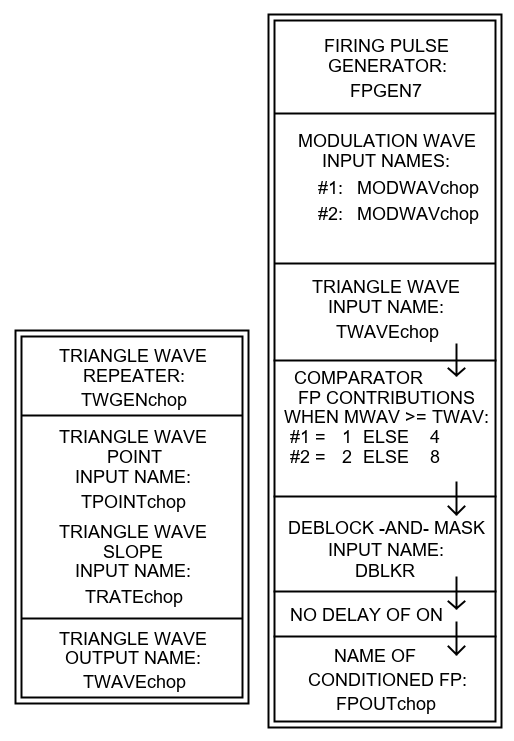
\includegraphics[height=7.5cm,width=5.5cm]{Diagrams/Appendix_A/Chopper_circuit_firing.PNG}
  \caption{Triangular wave repeater and Firing pulse generator for DC circuit}
  \label{fig:Chopper_circuit_firing}
\end{subfigure}
\caption{Chopper circuit in small time step block}
\label{fig:Chopper_circuit_valve_firing}
\end{figure}

\section{Grid Side Converter model}
\gls{GSC} also uses a three-level \gls{VSC} similar to the \gls{MSC}. The \gls{GSC} also uses \gls{PWM} technique for gating, and the points and slope for the triangular wave are created by the \gls{PLL} as shown in Figure \ref{fig:PLL_model}. The \gls{PLL} block plays a significant role in the entire network as it computes the phase angle of the space vector that defines the synchronization of the rotating \gls{dq} frame with the abc frame. The input for the \gls{PLL} is the three-phase voltage at the \gls{PCC}, and the angle is defined such that the d-axis aligns with the grid voltage and q-axis voltage is zero. This is done to achieve decoupled control of the two axes. Thereby, d-axis provides control of active power, and q-axis provides control of reactive power. The proportional and integral gains need to be defined in the \gls{PLL} block. The influence of these parameters in a grid dominated with \gls{PE} is an ongoing topic of research.

The slope and points for the triangular wave repeater are also generated in Figure \ref{fig:PLL_model}. The frequency of the carrier wave is chosen to be 19 times the nominal frequency (19*50 Hz). Therefore, the points would be 2*19*50 Hz if x = 0 and -2*19*50 Hz if x = 1. The angle is also multiplied by 19 and is between 0 and 2$\pi$, hence has to be divided by 2$\pi$ to achieve points between 0 and 1. The triangular wave repeater and the firing pulse generator for the \gls{GSC} are similar to that of the \gls{MSC} and are shown in Figure \ref{fig:Firing_blocks_GSC}. The numbers denominated for the three-phases of \gls{GSC} are 1,2 and 3 respectively.


\begin{figure}[H]
\centering
%\hspace*{-1.2cm}
    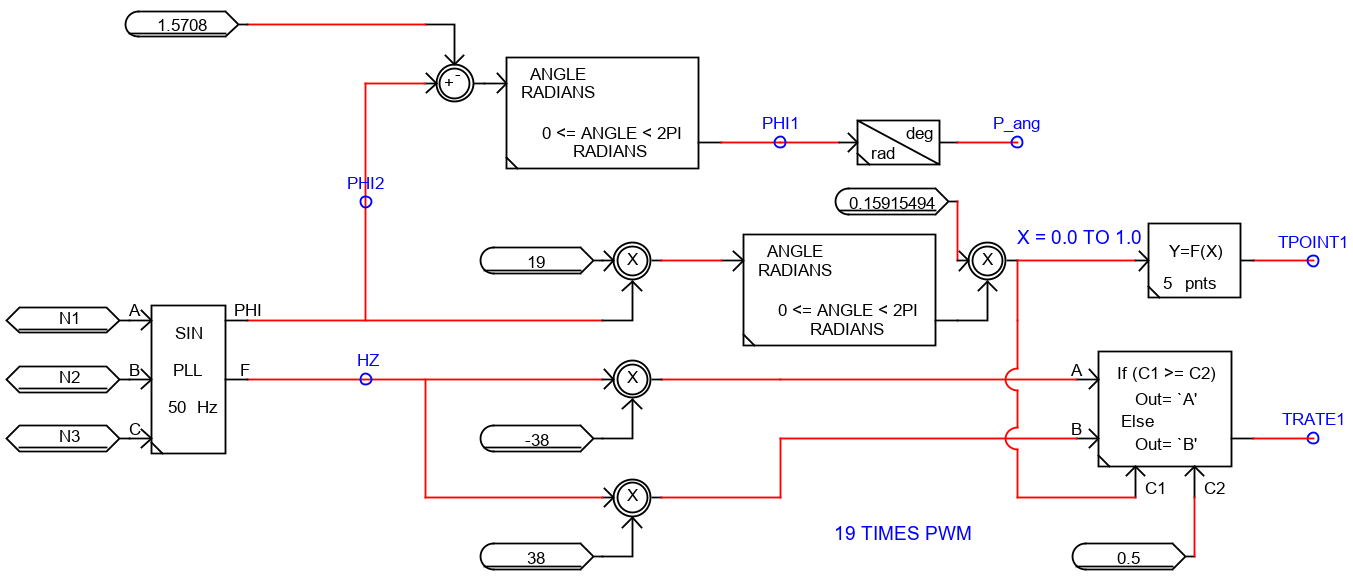
\includegraphics[height = 7cm,width = 15.5cm]{Diagrams/Appendix_A/PLL_model.PNG}
    \caption{PLL circuit, points and slope for triangular wave generation}
    \label{fig:PLL_model}
\end{figure}

\begin{figure}[H]
\centering
%\hspace*{-1.2cm}
    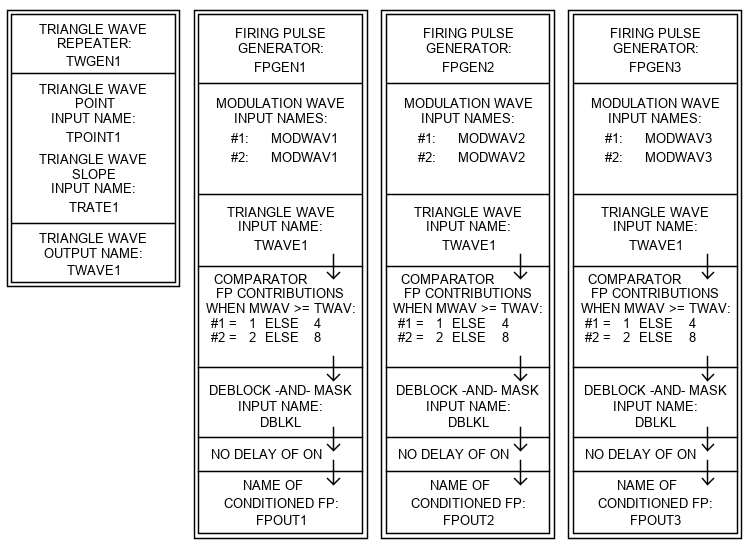
\includegraphics[height = 7.5cm,width = 9.5cm]{Diagrams/Appendix_A/Firing_blocks_GSC.PNG}
    \caption{Triangular wave repeater and Firing pulse generator for GSC}
    \label{fig:Firing_blocks_GSC}
\end{figure}

The \gls{GSC} control block has the abc to \gls{dq} transformation and vice versa, of \gls{PCC} voltages and currents, measurement of \gls{PCC} voltage in p.u. and the measurement of \gls{DC} voltage in p.u., as shown in Figure \ref{fig:GSC_Control_RSCAD_1}. The generation of the gating pulses are similar to the \gls{MSC} control. The outer and inner control loop structure of the implemented \gls{DVC} is illustrated in Figure \ref{fig:GSC_Control_RSCAD_2}.

\begin{figure}[H]
\centering
%\hspace*{-1.2cm}
    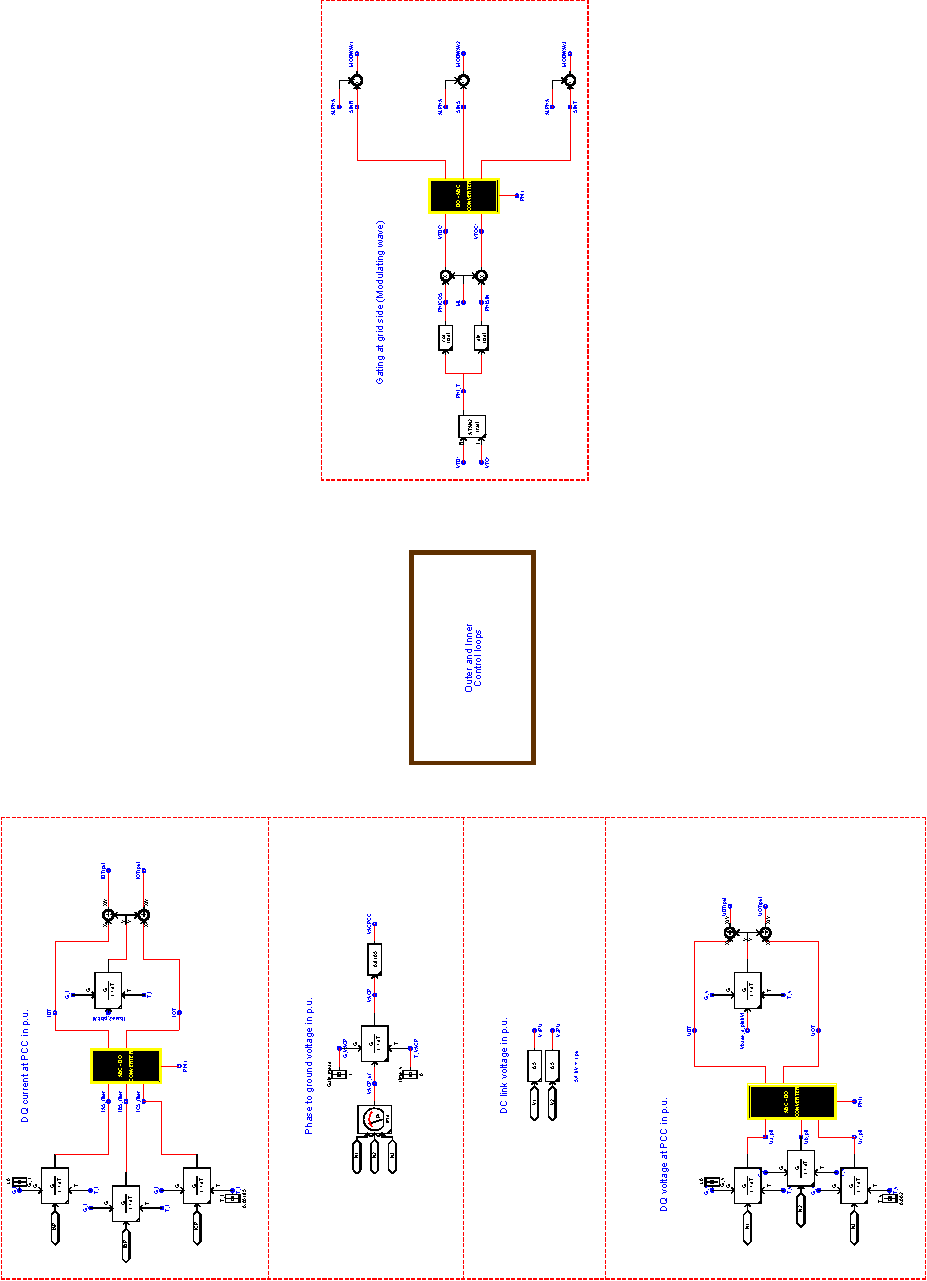
\includegraphics[height = 22cm,width = 14.5cm]{Diagrams/Appendix_A/GSC_Control_RSCAD_1.pdf}
    \caption{GSC control}
    \label{fig:GSC_Control_RSCAD_1}
\end{figure}

\begin{figure}[H]
\centering
%\hspace*{-1.2cm}
    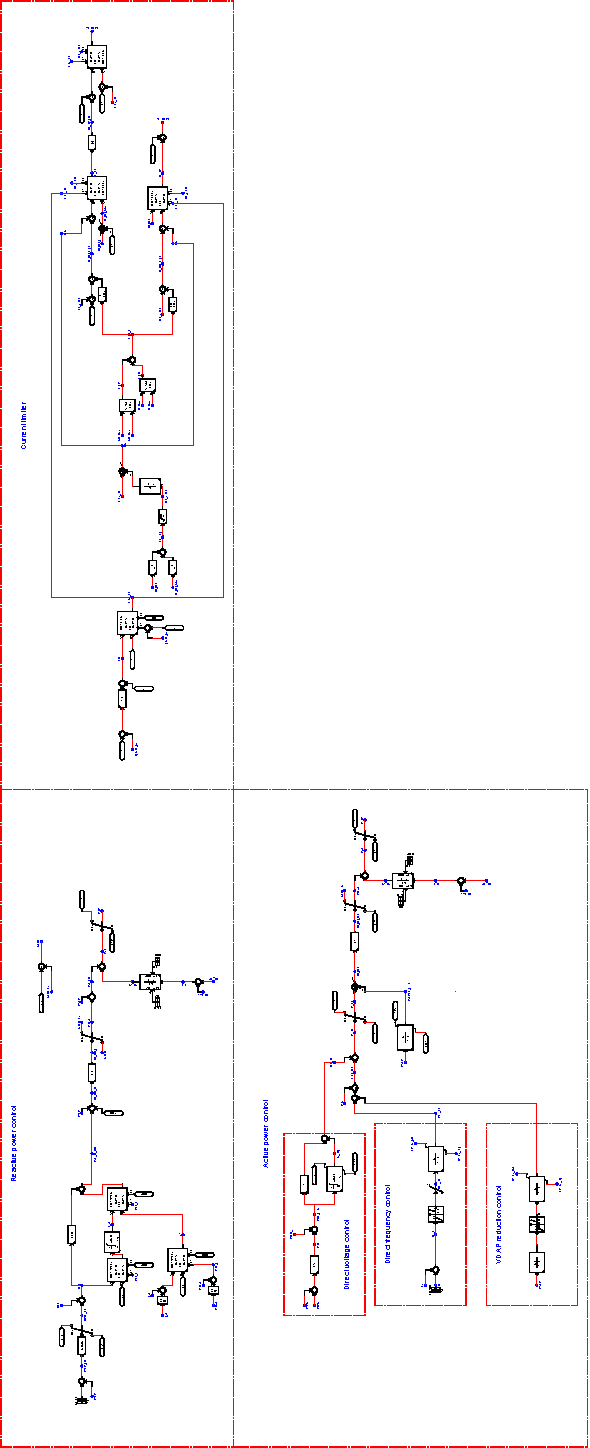
\includegraphics[height = 22cm,width = 12.5cm]{Diagrams/Appendix_A/GSC_Control_RSCAD_2.pdf}
    \caption{DVC representation in RSCAD}
    \label{fig:GSC_Control_RSCAD_2}
\end{figure}

\section{PowerFactory model}\label{pfd_model_appen}

\begin{figure}[H]
\centering
%\hspace*{-1.2cm}
    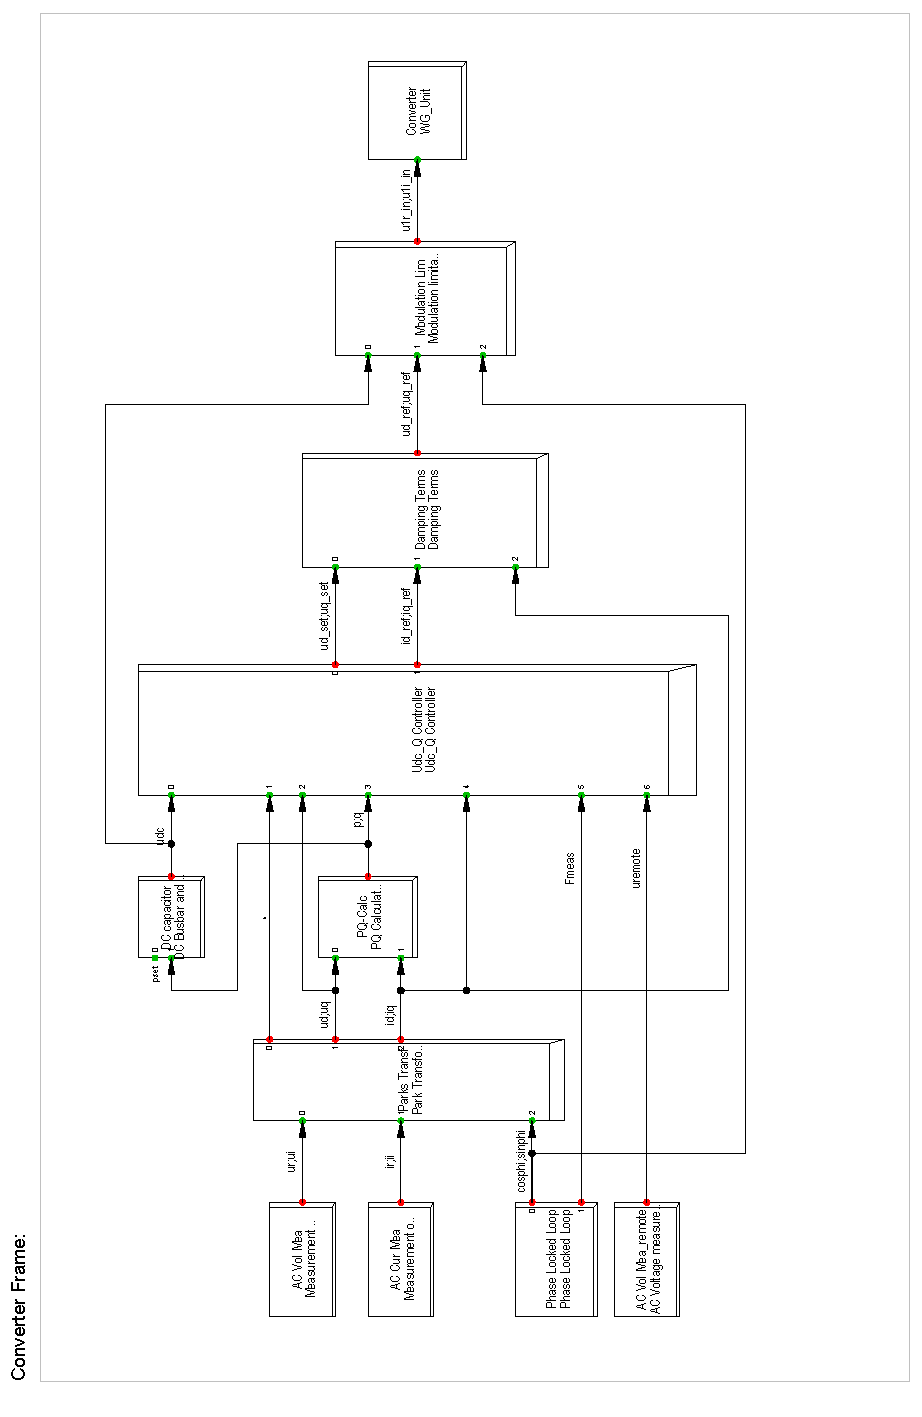
\includegraphics[height = 22cm,width = \textwidth]{Diagrams/Appendix_A/FSC_PFD.pdf}
    \caption{FSC representation in PowerFactory \cite{erlich_description_nodate}}
    \label{fig:FSC_PFD}
\end{figure}

\begin{figure}[H]
\centering
%\hspace*{-1.2cm}
    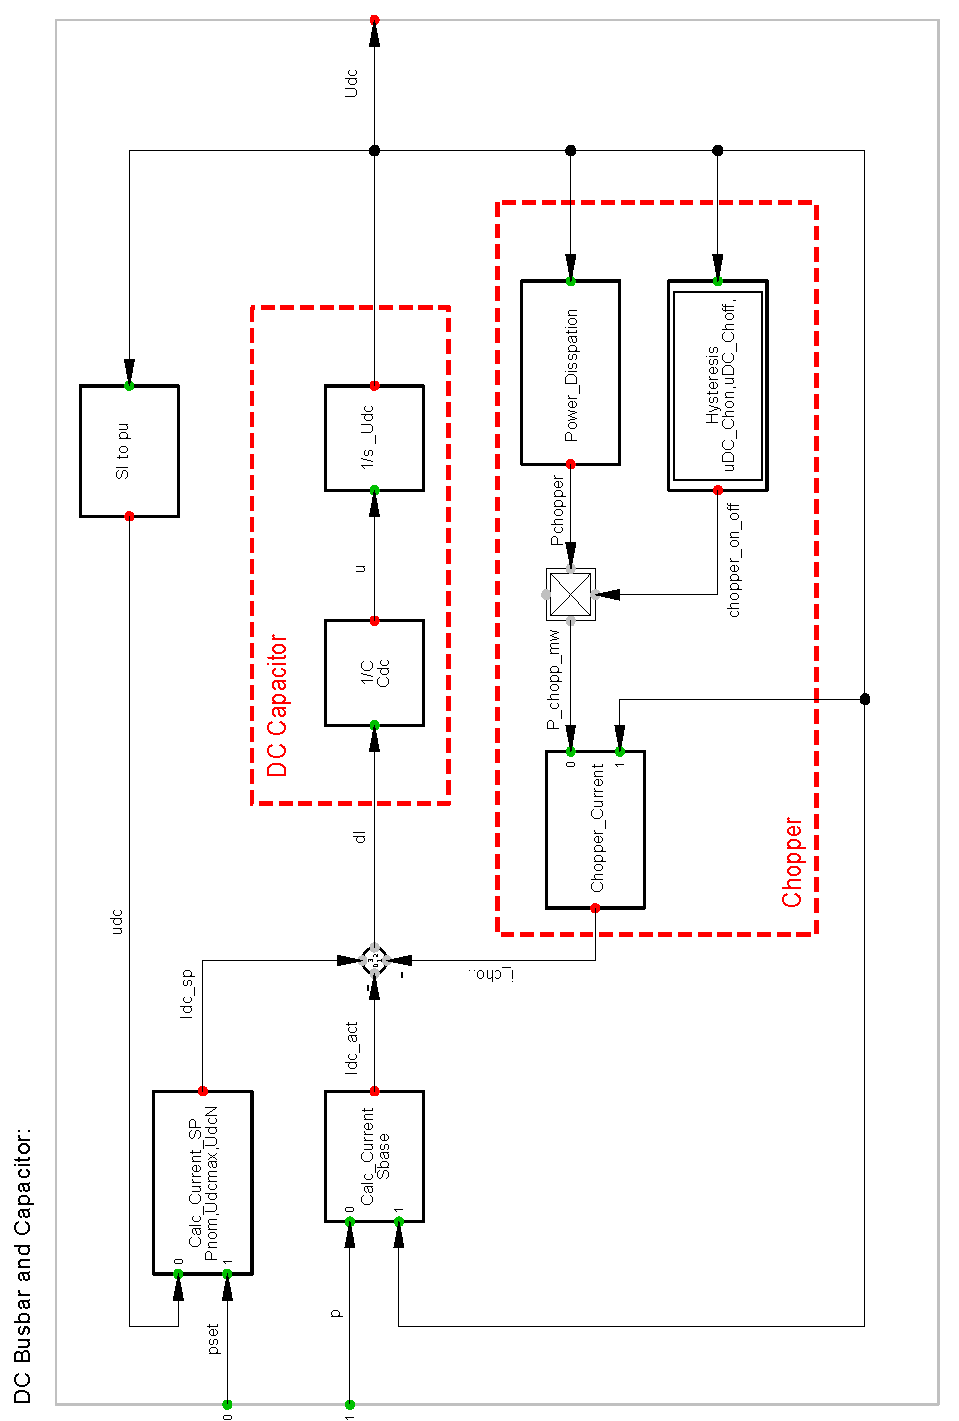
\includegraphics[height = 24cm,width =\textwidth]{Diagrams/Appendix_A/DC_bus_PFD.pdf}
    \caption{DC bus representation in PowerFactory \cite{erlich_description_nodate}}
    \label{fig:DC_bus_PFD}
\end{figure}

\begin{figure}[H]
\centering
%\hspace*{-1.2cm}
    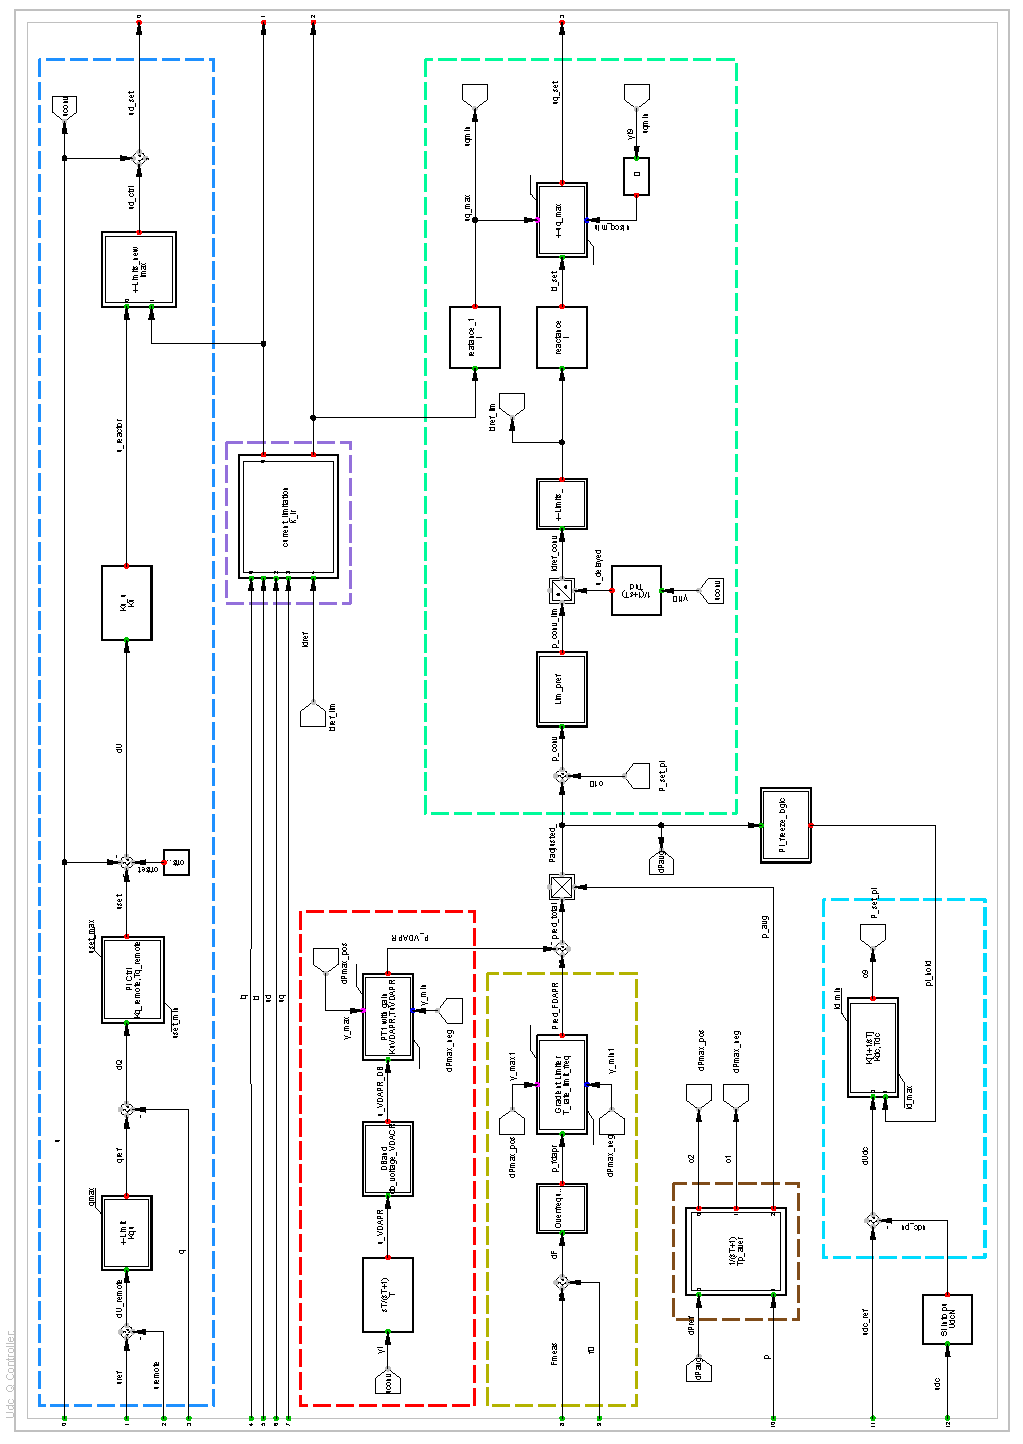
\includegraphics[height = 24cm,width =\textwidth]{Diagrams/Appendix_A/Udc_controller_PFD.pdf}
    \caption{DVC representation in PowerFactory \cite{erlich_description_nodate}}
    \label{fig:Udc_controller_PFD}
\end{figure}

\begin{figure}[H]
\centering
%\hspace*{-1.2cm}
    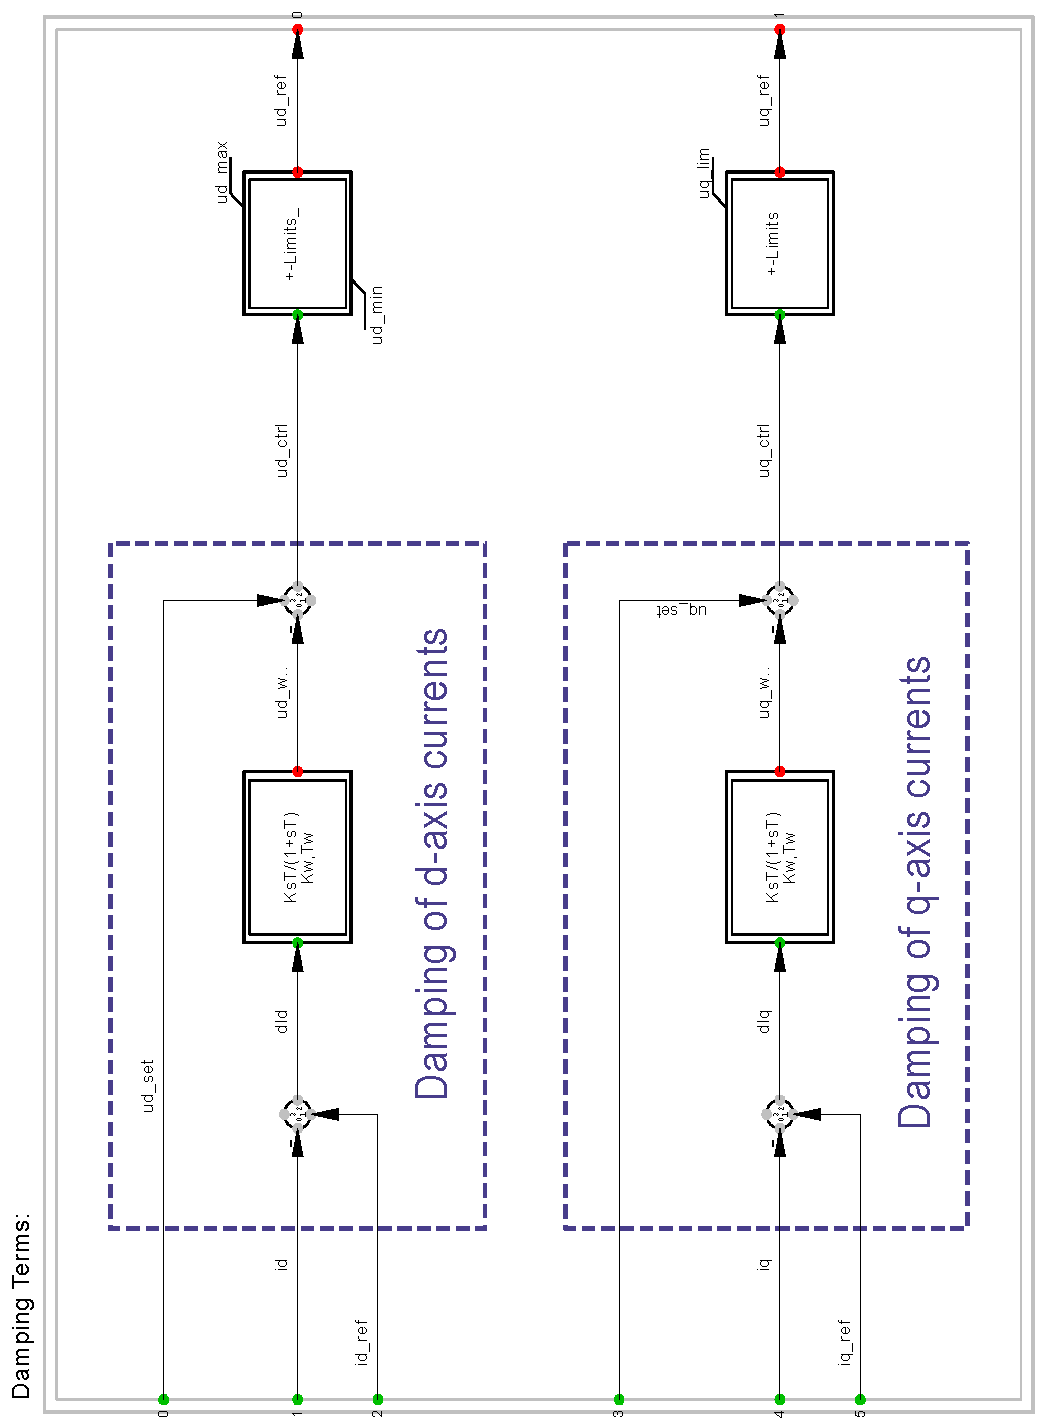
\includegraphics[height = 17cm,width =15cm]{Diagrams/Appendix_A/Damping_terms_PFD.pdf}
    \caption{Washout filter representation in PowerFactory \cite{erlich_description_nodate}}
    \label{fig:Damping_terms_PFD}
\end{figure}